
\todo[inline]{En ting å tenke på gjennom hele denne seksjonen er hvorfor du introduserer et konsept/en modell og hvem man skriver for. }

\todo[inline]{Her snakker vi om hvorfor vi introduserer tingene vi gjør. Litt om linja vi ønsker å legge oss på, den logiske oppbygningen i seksjonen etc.}

\section{Neural Networks}
Neural Networks (NNs), the cornerstone of many modern artificial intelligence applications, are computational models inspired by the human brain. They consist of interconnected groups of artificial neurons, where each connection represents a synaptic strength or weight. These weights are adjusted through a process known as learning. 

\todo[inline]{Ikke helt fornøyd. Legge ved en kilde på hvor de ble introduser første gang. Hvem som definerte og når?}


\subsection{Structure of Neural Networks}
\todo[inline]{Her må det komme en definisjon. Matriseformen er fin. Finn en god kilde på det.}
Typically, NNs are structured in layers, including:
\begin{itemize}
    \item \textbf{Input Layer:} This layer receives the raw input signal for the neural network.
    \item \textbf{Hidden Layers:} One or more layers where computation occurs through a system of weighted connections. These layers perform non-linear transformations of the inputs entered into the network.
    \item \textbf{Output Layer:} This layer produces the final output of the neural network.
\end{itemize}

\begin{figure}[H]
    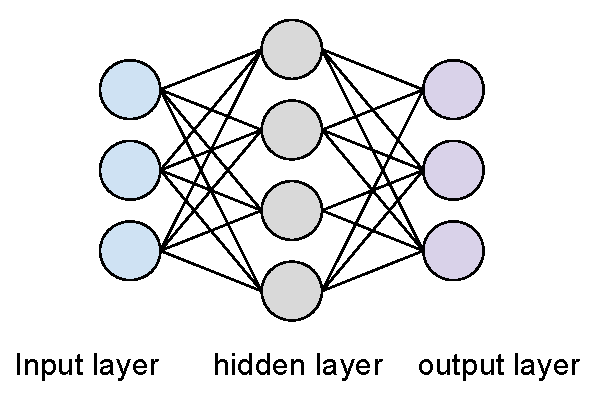
\includegraphics[scale=0.7]{figures/figure-pdf/NN.pdf}
    \caption{Simple neural network consisting of a single hidden layer.}
\end{figure}

\subsection{Learning in Neural Networks}
\todo[inline]{Her vil jeg egentlig at du tydelig snakker om gradient descent, og varianter av algoritmen. Referer til en kilde som går gjennom gradient descent i detalj}
The learning process involves adjusting the weights of the connections in the network through a process known as backpropagation, which calculates the gradient of the loss function with respect to the neural network's weights.


\subsection{Activation Functions}
\todo[inline]{Her bør det refereres til definisjonen av et NN. Nevne hvorfor det er rimelig at NN med ikke-lineær aktiveringsfunksjon kan approksimere mange ting:  http://www.vision.jhu.edu/teaching/learning/deeplearning18/assets/Cybenko-89.pdf}
Non-linear activation functions play a key role in NNs by introducing non-linear properties to the network. This non-linearity is essential because most real-world data is non-linear, meaning it can't be represented accurately with just a straight line.
The most common activation functions are sigmoid, tanh, and Rectified Linear Unit (ReLU).


ReLU has become a industry standard due to its simplicity and efficiency in backpropagation. It is expressed as: $ReLu(x) = \text{max}(0, x)$, with a simple gradient 1 for positive inputs and 0 for non-positive. 
In addition to its simplicity it is more efficient at preventing vanishing gradients compared to sigmoid and tanh \cite{ReLuGrad}. 

\subsection{Supervised and unsupervised learning}
Using a neural network \todo{Heller start med "In machine learning"??} there are two key learning paradigms. Supervised and unsupervised learning. Supervised learning refers to a learning process where the network has access to pre-labelled inputs which acts as targets.
For each training example there will be a set of input values alongside a designated output value, which is often human labeled.
A typical example is classification, where we measure how well the network performes by how well it classifies labels.\todo[inline]{Klassifisering er jo ikke supervised eller unsupervised? Definer klart hva supervised er, og så hva unsupervised er. Så kom med et klart eksempel på hver. Snakk også gjerne om hvor mye mer utbredt supervised er enn unsupervised.}

For unsupervised learning the training set does not include any labels, therefor we are limited to looking at how well the model minimizes or maximizes an assosiated cost function. \todo[inline]{Loss function? dette er første gang det nevnes. Definitivt verdt å definere sammen med "learning"}


\section{Convolutional Neural Networks, CNN}
\todo[inline]{Dette avsnittet er en direkte kopi fra https://www.deeplearningbook.org/contents/convnets.html}
Convolutional Neural Networks (CNNs)\cite{CNNs} \todo{riktig kilde?} are a specialized kind of neural network using convolutional layers and pooling for processing data that has a grid like topology . Examples include timeseries data, which can be thought of as a 1 dimensional grid taking samples at regular time intervals, and image data, which is a 2 dimensional grid of pixels. 

\subsection{Convolutional layers}
\todo[inline]{Ville skrevet mer i symboler her. Matematisk definert diskret konvulosjon? Lettere å snakke om K som en kjerne da.}
% \todo{https://en.wikipedia.org/wiki/Kernel_image_processing}


What characterizes a CNN is the use of a mathematical operation called convolution, which is a special kind of linear operation. The convolution leverages the spatial or temporal structure of the data by enforcing a local connectivity pattern between neurons of adjacent layers.
The parameters of the convolutional layers are composed of a set of learnable filters or kernels, which have a small receptive field, but is applied to all of the input data. This is achieved by computing the dot product between the entries of the filter and the input, producing a activation map of that filter.
As a result the network learns filters that activate when they see some specific type of feature at some spacial or temporal position in the input. 

\begin{center}
    \begin{figure}[H]
    \begin{tikzpicture}[
        2d-arr/.style={matrix of nodes, row sep=-\pgflinewidth, column sep=-\pgflinewidth, nodes={draw}}
      ]
    
      \matrix (mtr) [2d-arr] {
      0 & 1 & 1 & |[fill=orange!30]| 1 & |[fill=orange!30]| 0 & |[fill=orange!30]| 0 & 0\\
      0 & 0 & 1 & |[fill=orange!30]| 1 & |[fill=orange!30]| 1 & |[fill=orange!30]| 0 & 0\\
      0 & 0 & 0 & |[fill=orange!30]| 1 & |[fill=orange!30]| 1 & |[fill=orange!30]| 1 & 0\\
      0 & 0 & 0 & 1 & 1 & 0 & 0\\
      0 & 0 & 1 & 1 & 0 & 0 & 0\\
      0 & 1 & 1 & 0 & 0 & 0 & 0\\
      1 & 1 & 0 & 0 & 0 & 0 & 0\\
      };
    
      \node[below=of mtr-5-4] {$\mathbf I$};
    
      \node[right=0.2em of mtr] (str) {$*$};
    
      \matrix (K) [2d-arr, right=0.2em of str, nodes={draw, fill=teal!30}] {
        1 & 0 & 1 \\
        0 & 1 & 0 \\
        1 & 0 & 1 \\
      };
      \node[below=of K-3-2] {$\mathbf K$};
    
      \node[right=0.2em of K] (eq) {$=$};
    
      \matrix (ret) [2d-arr, right=0.2em of eq] {
      1 & 4 & 3 & |[fill=blue!80!black!30]| 4 & 1\\
      1 & 2 & 4 & 3 & 3\\
      1 & 2 & 3 & 4 & 1\\
      1 & 3 & 3 & 1 & 1\\
      3 & 3 & 1 & 1 & 0\\
      };
      \node[below=of ret-4-3] {$\mathbf{I * K}$};
    
      \draw[dashed, teal] (mtr-1-6.north east) -- (K-1-1.north west);
      \draw[dashed, teal] (mtr-3-6.south east) -- (K-3-1.south west);
    
      \draw[dashed, blue!80!black] (K-1-3.north east) -- (ret-1-4.north west);
      \draw[dashed, blue!80!black] (K-3-3.south east) -- (ret-1-4.south west);
    
      \foreach \i in {1,2,3} {
          \foreach \j in {4,5,6} {
              \node[font=\tiny, scale=0.6, shift={(-1.2ex,-2ex)}] at (mtr-\i-\j) {$\times \pgfmathparse{int(mod(\i+\j,2))}\pgfmathresult$};
            }
        }
    \end{tikzpicture}
    \caption{Example of convolutional operation. $\mathbf{I}$ is the input, $\mathbf{K}$ is the kernel and $\mathbf{I} * \mathbf{K}$ is the activation map. Illustration taken from the Random TikZ collection\cite{RiebesellTikZ2022}}
    \end{figure}
    \end{center}
    

In a convolutional layer, the configuration involves not only the selection of the filter (or kernel) size but also the specification of the stride length and the padding. The stride defines the number of units the filter shifts over the input data for each convolution operation. A stride of one moves the filter one unit at a time, capturing fine-grained information, while larger strides can speed up the computation and provide a more global view of the input data, albeit with reduced spatial resolution.
This reduction in spacial resolution is necessary for tasks like compression which we will discuss in the encoder section.

\subsection{Pooling}
\todo[inline]{Downsampling is a good word.}
A pooling layer is in essence a filter using a specified operation to reduce dimensionality. The pooling layer works similarely as a convolutional layer, they both slide through the temporal or spatial axis, computing a mathematical operation.

The most common pooling operations are:
\begin{itemize}
    \item \textbf{Max Pooling:} Selects the maximum element from the region of the feature map covered by the filter. This method is effective at capturing the presence of features.
    \item \textbf{Average Pooling:} Computes the average of the elements in the region of the feature map covered by the filter, which helps in smooth feature representation.
\end{itemize}

\begin{center}
    \begin{figure}[H]
    \begin{tikzpicture}[
        2d-arr/.style={
            matrix of nodes,
            nodes in empty cells,
            row sep=-\pgflinewidth,
            column sep=-\pgflinewidth,
            nodes={minimum size=1cm, draw, anchor=center, scale=0.7}
        },
        pool-box/.style={
            draw=red, thick, rounded corners
        },
        scale = 0.7
    ]

    \matrix (input) [2d-arr] {
         2 & 1 & |[fill=orange!30]| 3 & 0 \\
        |[fill=orange!30]| 4 &  3 & 2 &  1 \\
        0 & 2 & 1 & |[fill=orange!30]| 4 \\
        |[fill=orange!30]| 3 & 2 &  1 & 1 \\
    };

    \node[left=of input-2-1.west, anchor=center, rotate=90] {Input Feature Map};
    
    \matrix (output) [2d-arr, right=2cm of input] {
        |[fill=blue!30]| 4 & |[fill=blue!30]| 3 \\
        |[fill=blue!30]| 3 & |[fill=blue!30]| 4 \\
    };

    \node[right=of output-2-2.east, anchor=center, rotate=90] {Max Pooled Feature Map};

    \draw[pool-box] (input-1-1.north west) rectangle (input-2-2.south east);
    \draw[pool-box] (input-1-3.north west) rectangle (input-2-4.south east);
    \draw[pool-box] (input-3-1.north west) rectangle (input-4-2.south east);
    \draw[pool-box] (input-3-3.north west) rectangle (input-4-4.south east);

    \draw[->, thick] (input) -- (output) node[midway, above] {Max Pooling};

    \end{tikzpicture}
\caption{Illustration of a max pooling operation. The input feature map is reduced in size by applying a max pooling filter with size 2x2 (red boxes), which selects the maximum value in each filter region to produce the max pooled feature map.}
\end{figure}
\end{center}

Using a pooling layer in a neural network architecture helps the network to learn better feature representations. This is beneficial for enhancing the efficiency of convolutional filters.

\subsection{Architecture of CNNs}
A typical CNN architecture consists of the following layers:

\begin{itemize}
    \item \textbf{Convolutional Layer} — Applies the learnable filters on the input data, producing a activation map. Each filter detects different features by convolving with the input.
    \item \textbf{Activation Function} — Typically, a ReLU is applied to introduce non-linearity into the model, allowing it to learn more complex functions.
    \item \textbf{Pooling} — This layer reduces the spatial size of the representation, reducing the number of parameters and computation in the network, and hence, also controlling overfitting. 
    \item \textbf{Fully Connected Layer} — Neurons in a fully connected layer have full connections to all activations in the previous layer. Primarely used for processing the information obtained through the convolutional layers to perform a task like classification.
\end{itemize}


\section{Encoder}
\todo[inline]{Her ville jeg flyttet hele Encoder/Decoder og Projector delen til Methodology, og heller laget en seksjon her med Residual Networks som du kan referere til når du introduserer Encoder og Decoder i VQVAE sammenheng.}
The Encoder has the task of compressing the high-dimensional input data into a compact and manageable representation. It is a component of the Variational Auto-Encoder architecture, enabling the compression of input to latent variables.
The encoded data should capture important characteristics and features from the input data necessary for decompression while also removing unessesary and reduntant information. 
It operates by using a block like structure, where each block is designed to process the input data sequentially.

\subsection{Downsampling blocks}
Downsampling blocks are integral components within encoder architectures, facilitating the reduction of dimensionality of the feature maps. Based on the principles of CNNs the downsampling is achieved through a convolutional layer, that not only detects patterns within the input data but also strategically reduces the dimensions of the input.
The convolutional layer applies filters to the input, creating activation maps that highlight significant features. By adjusting the stride of the convolution, the layer can downsample the input, distilling the information into a more compact form. 

Following the convolutional layer, batch normalization is employed. This technique normalizes the output of the convolution by adjusting and scaling the activations. It allows the network to use higher learning rates, as it reduces the internal covariate shift which in turn makes the learning process more efficient and stable, as described by Ioffe and Szegedy\cite{batchnorm}.

\subsection{Residual block}
To enhance the encoder's ability to learn complex patterns and facilitate the training of deeper networks, residual blocks are integrated. These blocks, which were first introduced by He et al. in their paper on deep residual learning \cite{ResLearn}, incorporate shortcut connections that bypass one or more layers. 
The primary advantage of these shortcuts is to allow gradients to flow directly through the network, mitigating the vanishing gradient problem that often plagues deep neural networks. 

\begin{figure}[H]
    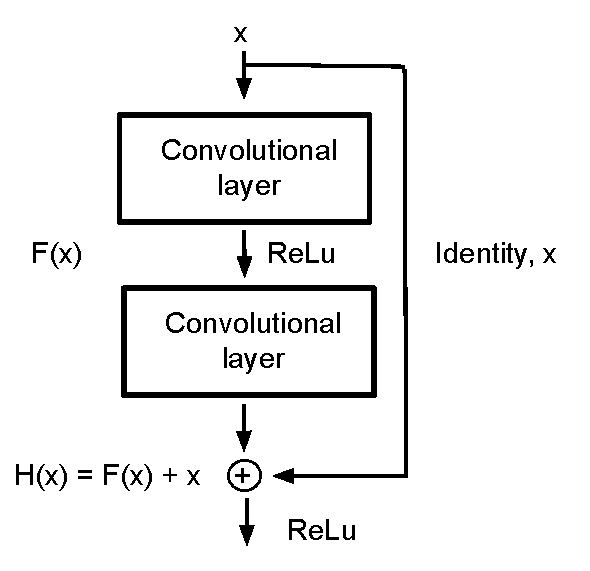
\includegraphics[scale=0.6]{figures/figure-pdf/Resnet.pdf}
    \caption{Illustration of the Resnet block from He et al's original paper\cite{ResLearn} }
\end{figure}


\subsection{Encoder Architecture}
The complete encoder architecture comprises a sequence of downsampling blocks, each further distilling the data. This is then followed by a series of Residual blocks to form deeper representations efficiently. The overall structure is sequential, with each block building upon the previous one to gradually reduce the input data's dimensionality while capturing
patterns and important features. The number of downsampling blocks is determined by a downsampling rate which is dependent of the size of the input data, and the amount of compression needed for the encoding task.

\begin{figure}[H]
    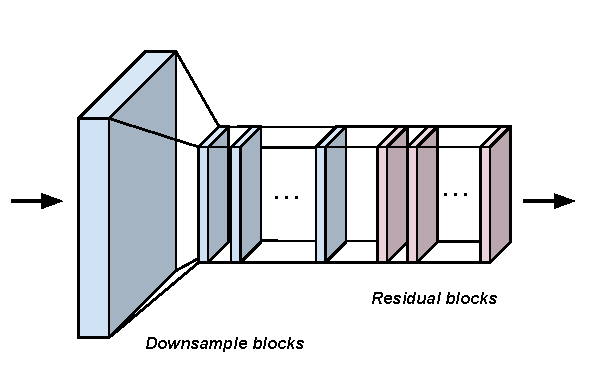
\includegraphics[scale=0.8]{figures/figure-pdf/Encoder.pdf}
    \caption{Illustration of the Encoder architecture used in the VQVAE implementation. The first downsample block reduces the dimensionality, followed by further downsample blocks to capture important features.}
\end{figure}

\section{Decoder}
While the encoder is responsible for data compression, the decoder is responsible for decompression. Instead of reducing the dimensions of the data, it will upsample it to a higher dimensional space.

\subsection{Upsampling Blocks}
Contrary to the encoder's downsampling blocks, the decoder employs upsampling blocks designed to incrementally reconstruct the higher-dimensional data from the lower-dimensional representation.  
The upsampling process is achieved through the use of transposed convolutional layers, often referred to as deconvolutional layers. These layers effectively reverse the operation of convolution by learning to expand a compressed feature map onto a larger spatial canvas.
The transposed convolutions apply filters in a manner that distributes the encoded feature values over a higher-resolution grid, interpolating additional data points as necessary to achieve the desired output size.
This process not only increases the spatial dimensions but also refines the feature map to recover details that were compressed during encoding.
Following the transpose convolutional layer the upsample block uses batch normalization and ReLu activation function.


\subsection{Decoder Architecture}
The decoder's architecture is characterized by a series residual blocks followed by upsampling blocks that progressively restore the data's dimensionality. The number of upsampling blocks is the same as number of downsampling blocks in the encoder. 

\section{Self Supervised Learning, SSL}
Self-supervised learning (SSL) is a form of unsupervised learning where the data itself provides the supervision. SSL algorithms learn to predict unobserved or hidden parts of the input from observed parts.
This is achieved trough carefully designed loss functions, which enforce the learning of usefull features by solving pretext tasks. Modern mainstream SSL frameworks can be divided into two categories, contrastive and non-contrastive learning.

\subsection{Contrastive Learning in SSL}
Contrastive learning is a popular method in SSL, particularly for learning visual representations. It relies on contrasting positive pairs (similar or related data points) against negative pairs (dissimilar or unrelated data points). 
The intuition is to learn embeddings such that similar samples are closer to each other in the embedding space, while dissimilar ones are farther apart.
Several prominent contrastive learning methods, such as MoCo\cite{MoCo} and SimCLR\cite{SimCLR}, effectively utilize positive and negative pairs to learn contrasted representations.

\subsection{Non-Contrastive Learning in SSL}
Non-Contrastive learning methods in SSL, by contrast, does not depend on negative pairs. Instead, these approaches aim to learn representations by encouraging similarity between different augmented views of the same data point. 
This approach is based on the principle that different transformations of the same data should yield similar representations, thereby ensuring consistency and robustness in the learned features.

Notable non-contrastive methods include BYOL (Bootstrap Your Own Latent)\cite{BYOL} and Barlow Twins \cite{Barlow}.

\subsection{The Role of Siamese Networks in SSL}
Siamese networks\cite{Siamese} is a neural network architecture designed for specialized tasks that require the comparison of input pairs. The defining characteristics of these networks is the dual-branch structure, where two identical sub-networks with shared parameters process two seperate inputs.
The outputs of the sub networks, often refered to as twin embeddings, are then brought togheter to evaluate the degree of similarity or difference.

Many modern SSL approaches base their architecture on the siamese network as it is efficient for teaching a sub network to discriminate between different classes or types of data as explored by Lee and Aune in their paper on SSL methods on timeseries \cite{SSLs}


\begin{figure}[H]
    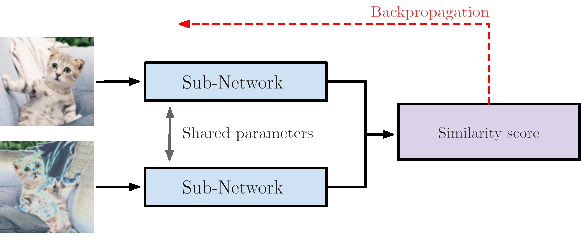
\includegraphics[scale=1]{figures/figure-pdf/Siamese.pdf}
    \caption{ Example of a non contrastive siamese network using augmented views. Here the images are processed to calculate a similarity score, the backpropagation arrow indicates that the similarity score is then used to update the weights of the sub network. Pictures taken from \url{www.pexels.com}}
\end{figure}

\subsection{Projector}
The projector serves as a component in the sub-network component of siamese networks.
Its main function is to transform a lower-dimensional encoded representation into a higher dimensional space suited for a SSL loss function. Common SSL techniques using projectors 
include BYOL, SimCLR and Barlow Twins.


\subsubsection{Projector architecture}
The projector architecture is designed with the objective of expanding the number of features through fully connected layers. The arcitecture used in this methology consist of the following components.
\todo{Bit vague}
\begin{itemize}
    \item \textbf{Global max pooling.} Condenses the input encodings into a condensed and robust set of features. This helps distill the most salient aspects of the encoded data.
    \item \textbf{Fully connected layers}. Broadens the dimensions and learns weights and biases that emphasize differences 
    \item \textbf{batch normalization}
    \item \textbf{ReLu activation function}
\end{itemize}


\section{Additional Machine Learning Algorithms}
\todo[inline]{Jeg er strengt tatt ikke sikker på om du trenger å ha med dette. SVM, KNN og KMeans er jo kjent fra bachelornivå. Vi skal skrive for en mastersudent i stat/ML}
\subsection{Support Vector Machines, SVM}
Support Vector Machines (SVM) is a supervised machine learning algorithm widely used for classification and regression tasks. The core idea of SVM is to establish an optimal hyperplane that maximizes the margin between different class labels. This approach is effective in high-dimensional spaces, addressingthe curse of dimensionality through its dependence on support vectors.
These support vectors are a critical subset of the training data that influences the construction of the decision boundary. SVM's adaptability is further enhanced by its capability to incorparate various kernel functions, such as linear and radial basis functions, to suit different types
of data distributions. The foundation of SVM is largely based on the work done by Vapnik et al\cite{svm}.
\begin{figure}[H]
    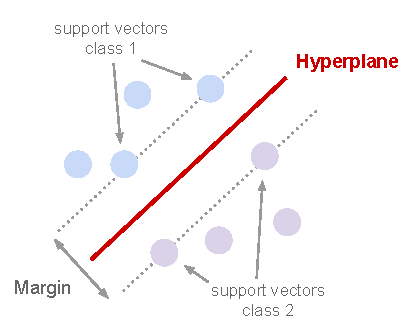
\includegraphics[scale=0.8]{figures/figure-pdf/SVM.pdf}
    \caption{Vizualisation of the hyperplane, margin and support vectors in a SVM procedure.}
\end{figure}


\subsection{K-Neares Neighbors, KNN}
K-Nearest Neighbors (KNN) is a versatile supervised learning algorithm that classifies data points based on the majority class of their K nearest neighbors.
It operates under the assumption that similar data points are likely to be close in proximity. One of the key strengths of KNN is its simplicity and effectiveness in classification tasks. 
However the KNNs performance is significally impacted by the choice of K and the distance metric used, visualized in fig \ref{fig:knn}.
The choice of K is often determined by techniques like cross validation.

\begin{figure}[H]
    \centering
    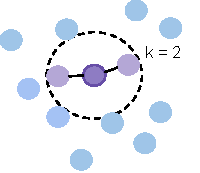
\includegraphics[width=0.3\textwidth]{figures/figure-pdf/2NN.pdf}
    \hspace{1cm}
    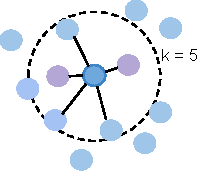
\includegraphics[width=0.3\textwidth]{figures/figure-pdf/5NN.pdf}
    \caption{Classification of middle point in a KNN procedure. For $k=2$ the majority vote is purple while for $k=5$ it is blue.}
    \label{fig:knn}
\end{figure}

\subsection{KMeans and Silhouette Score}
K-Means is a popular unsupervised learning algorithm used primarely for clustering.
Its goal is to partition the data into K distinct clusters, each represented by its centroid, which is the mean of the points in the cluster.
The algorithm iteratively assigns each data to the neares cluster, based on the Euclidian distance to the centroid, and then recalculates the centroids. 
This process repeats until the centroids stabilize or a certain iteration criteria is met. 

The Silhouette Score is a metric for evaluating the effectiveness of the clustering process. It measures how similar an object is to its own cluster (cohesion) compared to other clusters (separation).
The score ranges from -1 to 1, where a high value indicates that the object is well matched to its own cluster and poorly matched to neighboring clusters.

\begin{itemize}
    \item \textbf{Cohersion (a)}. It measures the average distance of the data point from all other points in the same cluster. \\
    \item \textbf{Seperation (b)}. It is the average distance of the data point to the points in the nearest cluster that the data point is not apart of.
\end{itemize}

The formula for the Silhouette score of a single data point ($i$) is given by:
\begin{equation}
    S_i = \frac{b_i-a_i}{\text{max}(a_i, b_i)}
\end{equation}

The overall silhouette score, $S$, for a dataset is the mean of the silhouette score of each data point.
\begin{figure}[H]
    \centering
    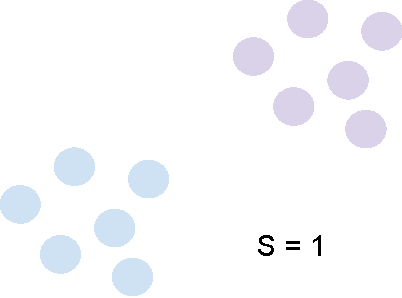
\includegraphics[width=0.3\textwidth]{figures/figure-pdf/Shigh.pdf}
    \hspace{1cm}
    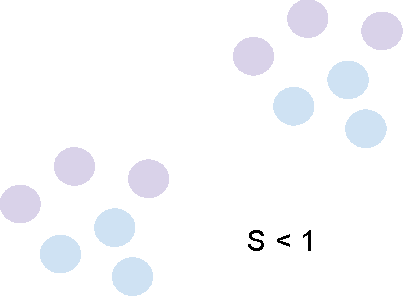
\includegraphics[width=0.3\textwidth]{figures/figure-pdf/Slow.pdf}
    \caption{Illustration of the silhuette score metric applied. On the left we see well seperated clusters with a silhouette score equal to 1. On the right a not so well seperation, giving a silhouette score less than 1.}
    \label{fig:knn}
\end{figure}

\section{Representation Learning}

\do{https://www.deeplearningbook.org/contents/representation.html}
